% Options for packages loaded elsewhere
% Options for packages loaded elsewhere
\PassOptionsToPackage{unicode}{hyperref}
\PassOptionsToPackage{hyphens}{url}
\PassOptionsToPackage{dvipsnames,svgnames,x11names}{xcolor}
%
\documentclass[
  letterpaper,
  DIV=11,
  numbers=noendperiod]{scrartcl}
\usepackage{xcolor}
\usepackage{amsmath,amssymb}
\setcounter{secnumdepth}{5}
\usepackage{iftex}
\ifPDFTeX
  \usepackage[T1]{fontenc}
  \usepackage[utf8]{inputenc}
  \usepackage{textcomp} % provide euro and other symbols
\else % if luatex or xetex
  \usepackage{unicode-math} % this also loads fontspec
  \defaultfontfeatures{Scale=MatchLowercase}
  \defaultfontfeatures[\rmfamily]{Ligatures=TeX,Scale=1}
\fi
\usepackage{lmodern}
\ifPDFTeX\else
  % xetex/luatex font selection
\fi
% Use upquote if available, for straight quotes in verbatim environments
\IfFileExists{upquote.sty}{\usepackage{upquote}}{}
\IfFileExists{microtype.sty}{% use microtype if available
  \usepackage[]{microtype}
  \UseMicrotypeSet[protrusion]{basicmath} % disable protrusion for tt fonts
}{}
\makeatletter
\@ifundefined{KOMAClassName}{% if non-KOMA class
  \IfFileExists{parskip.sty}{%
    \usepackage{parskip}
  }{% else
    \setlength{\parindent}{0pt}
    \setlength{\parskip}{6pt plus 2pt minus 1pt}}
}{% if KOMA class
  \KOMAoptions{parskip=half}}
\makeatother
% Make \paragraph and \subparagraph free-standing
\makeatletter
\ifx\paragraph\undefined\else
  \let\oldparagraph\paragraph
  \renewcommand{\paragraph}{
    \@ifstar
      \xxxParagraphStar
      \xxxParagraphNoStar
  }
  \newcommand{\xxxParagraphStar}[1]{\oldparagraph*{#1}\mbox{}}
  \newcommand{\xxxParagraphNoStar}[1]{\oldparagraph{#1}\mbox{}}
\fi
\ifx\subparagraph\undefined\else
  \let\oldsubparagraph\subparagraph
  \renewcommand{\subparagraph}{
    \@ifstar
      \xxxSubParagraphStar
      \xxxSubParagraphNoStar
  }
  \newcommand{\xxxSubParagraphStar}[1]{\oldsubparagraph*{#1}\mbox{}}
  \newcommand{\xxxSubParagraphNoStar}[1]{\oldsubparagraph{#1}\mbox{}}
\fi
\makeatother


\usepackage{longtable,booktabs,array}
\usepackage{calc} % for calculating minipage widths
% Correct order of tables after \paragraph or \subparagraph
\usepackage{etoolbox}
\makeatletter
\patchcmd\longtable{\par}{\if@noskipsec\mbox{}\fi\par}{}{}
\makeatother
% Allow footnotes in longtable head/foot
\IfFileExists{footnotehyper.sty}{\usepackage{footnotehyper}}{\usepackage{footnote}}
\makesavenoteenv{longtable}
\usepackage{graphicx}
\makeatletter
\newsavebox\pandoc@box
\newcommand*\pandocbounded[1]{% scales image to fit in text height/width
  \sbox\pandoc@box{#1}%
  \Gscale@div\@tempa{\textheight}{\dimexpr\ht\pandoc@box+\dp\pandoc@box\relax}%
  \Gscale@div\@tempb{\linewidth}{\wd\pandoc@box}%
  \ifdim\@tempb\p@<\@tempa\p@\let\@tempa\@tempb\fi% select the smaller of both
  \ifdim\@tempa\p@<\p@\scalebox{\@tempa}{\usebox\pandoc@box}%
  \else\usebox{\pandoc@box}%
  \fi%
}
% Set default figure placement to htbp
\def\fps@figure{htbp}
\makeatother


% definitions for citeproc citations
\NewDocumentCommand\citeproctext{}{}
\NewDocumentCommand\citeproc{mm}{%
  \begingroup\def\citeproctext{#2}\cite{#1}\endgroup}
\makeatletter
 % allow citations to break across lines
 \let\@cite@ofmt\@firstofone
 % avoid brackets around text for \cite:
 \def\@biblabel#1{}
 \def\@cite#1#2{{#1\if@tempswa , #2\fi}}
\makeatother
\newlength{\cslhangindent}
\setlength{\cslhangindent}{1.5em}
\newlength{\csllabelwidth}
\setlength{\csllabelwidth}{3em}
\newenvironment{CSLReferences}[2] % #1 hanging-indent, #2 entry-spacing
 {\begin{list}{}{%
  \setlength{\itemindent}{0pt}
  \setlength{\leftmargin}{0pt}
  \setlength{\parsep}{0pt}
  % turn on hanging indent if param 1 is 1
  \ifodd #1
   \setlength{\leftmargin}{\cslhangindent}
   \setlength{\itemindent}{-1\cslhangindent}
  \fi
  % set entry spacing
  \setlength{\itemsep}{#2\baselineskip}}}
 {\end{list}}
\usepackage{calc}
\newcommand{\CSLBlock}[1]{\hfill\break\parbox[t]{\linewidth}{\strut\ignorespaces#1\strut}}
\newcommand{\CSLLeftMargin}[1]{\parbox[t]{\csllabelwidth}{\strut#1\strut}}
\newcommand{\CSLRightInline}[1]{\parbox[t]{\linewidth - \csllabelwidth}{\strut#1\strut}}
\newcommand{\CSLIndent}[1]{\hspace{\cslhangindent}#1}



\setlength{\emergencystretch}{3em} % prevent overfull lines

\providecommand{\tightlist}{%
  \setlength{\itemsep}{0pt}\setlength{\parskip}{0pt}}



 


\KOMAoption{captions}{tableheading}
\makeatletter
\@ifpackageloaded{caption}{}{\usepackage{caption}}
\AtBeginDocument{%
\ifdefined\contentsname
  \renewcommand*\contentsname{Table of contents}
\else
  \newcommand\contentsname{Table of contents}
\fi
\ifdefined\listfigurename
  \renewcommand*\listfigurename{List of Figures}
\else
  \newcommand\listfigurename{List of Figures}
\fi
\ifdefined\listtablename
  \renewcommand*\listtablename{List of Tables}
\else
  \newcommand\listtablename{List of Tables}
\fi
\ifdefined\figurename
  \renewcommand*\figurename{Figure}
\else
  \newcommand\figurename{Figure}
\fi
\ifdefined\tablename
  \renewcommand*\tablename{Table}
\else
  \newcommand\tablename{Table}
\fi
}
\@ifpackageloaded{float}{}{\usepackage{float}}
\floatstyle{ruled}
\@ifundefined{c@chapter}{\newfloat{codelisting}{h}{lop}}{\newfloat{codelisting}{h}{lop}[chapter]}
\floatname{codelisting}{Listing}
\newcommand*\listoflistings{\listof{codelisting}{List of Listings}}
\makeatother
\makeatletter
\makeatother
\makeatletter
\@ifpackageloaded{caption}{}{\usepackage{caption}}
\@ifpackageloaded{subcaption}{}{\usepackage{subcaption}}
\makeatother
\usepackage{bookmark}
\IfFileExists{xurl.sty}{\usepackage{xurl}}{} % add URL line breaks if available
\urlstyle{same}
\hypersetup{
  pdftitle={{[}FILL: Title of the paper{]}},
  pdfauthor={{[}FILL: Author One{]}; {[}FILL: Author Two{]}},
  pdfkeywords={{[}FILL: keyword 1{]}, {[}FILL: keyword 2{]}, {[}FILL:
keyword 3{]}},
  colorlinks=true,
  linkcolor={blue},
  filecolor={Maroon},
  citecolor={Blue},
  urlcolor={Blue},
  pdfcreator={LaTeX via pandoc}}


\title{{[}FILL: Title of the paper{]}}
\usepackage{etoolbox}
\makeatletter
\providecommand{\subtitle}[1]{% add subtitle to \maketitle
  \apptocmd{\@title}{\par {\large #1 \par}}{}{}
}
\makeatother
\subtitle{{[}FILL: Subtitle of the paper{]}}
\author{{[}FILL: Author One{]} \and {[}FILL: Author Two{]}}
\date{2026-04-15}
\begin{document}
\maketitle
\begin{abstract}
{[}FILL: Write your abstract here. Summarize the research question,
methods, key findings, and implications.{]}
\end{abstract}


\section{Introduction}\label{sec-introduction}

Understanding the determinants of economic growth across countries
remains a central question in development economics. Following the
seminal work of Keola, Andersson, and Hall (2015), a large empirical
literature has examined how initial conditions, physical and human
capital accumulation, and trade affect growth trajectories.

This paper uses a synthetic panel dataset of 40 countries over six
five-year periods (1990--2015) to investigate the determinants of GDP
per capita growth. We employ panel data fixed effects methods to account
for unobserved country-specific heterogeneity and common time shocks.

This study contributes to the literature in two ways. First, we provide
a multi-language reproducible workflow demonstrating panel data analysis
in Python, R, and Stata. Second, we show how modern tools can enhance
transparency in empirical research.

The rest of this article is organized as follows.
Section~\ref{sec-literature} provides an overview of the related
literature. Section~\ref{sec-data} introduces the data and methods.
Section~\ref{sec-results} presents the results and discussion. Finally,
Section~\ref{sec-conclusion} offers some concluding remarks.

\section{Related literature}\label{sec-literature}

The relationship between initial income and subsequent growth --- the
convergence hypothesis --- has been extensively studied since the
seminal work of Keola, Andersson, and Hall (2015). Recent advances in
panel data econometrics have enabled more nuanced analyses that control
for unobserved heterogeneity across countries\footnote{See also the
  World Bank regional development reports.}.

\section{Data and methods}\label{sec-data}

\subsection{Data}\label{data}

We use a balanced panel of 40 countries observed at five-year intervals
from 1990 to 2015 (240 country-period observations). The dataset
includes GDP per capita growth as the dependent variable and five
regressors: log initial GDP per capita (capturing convergence),
investment share, years of schooling, population growth, and trade
openness. Full details on data construction are provided in
\href{notebooks/notebook-01.qmd}{N1: Panel Data Analysis (Python)}.

The following figure shows the distribution of GDP growth rates across
the six time periods.

\begin{figure}[H]

\centering{

\pandocbounded{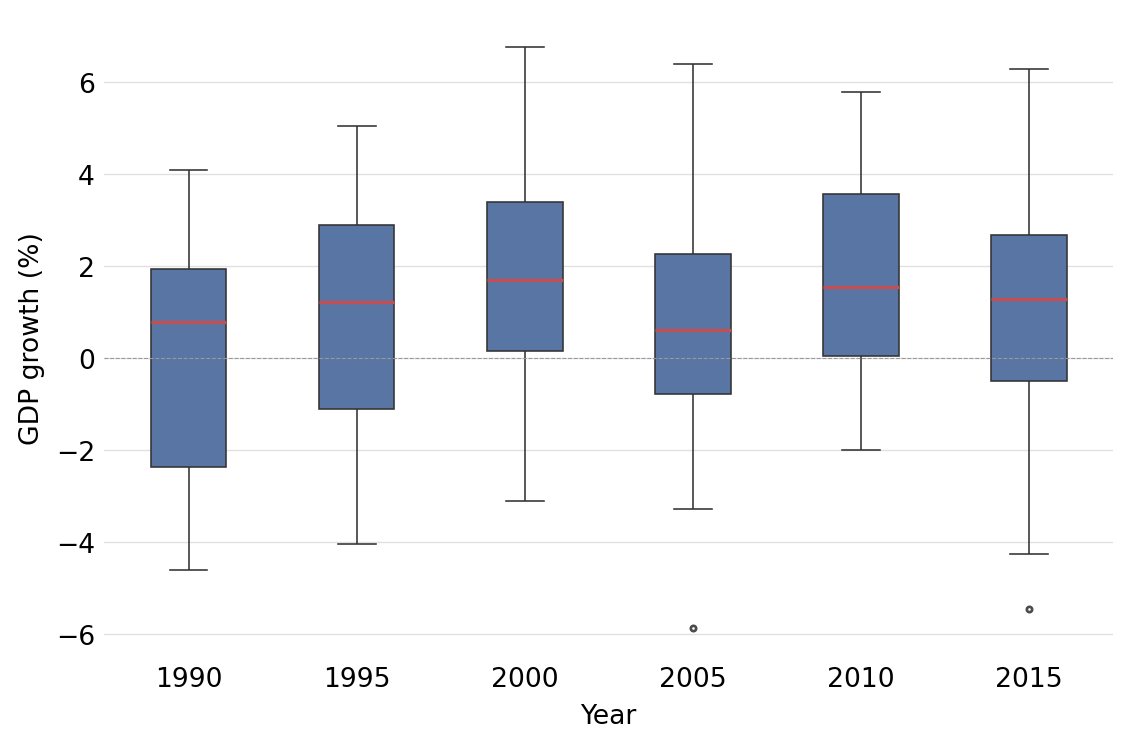
\includegraphics[keepaspectratio]{index_files/figure-latex/notebooks-notebook-01-fig-growth-time-output-1.png}}

}

\caption{\label{fig-growth-time}Distribution of GDP per capita growth
rates by period.}

\end{figure}%

The convergence hypothesis predicts a negative relationship between
initial income and subsequent growth. The following scatter plot
illustrates this pattern in our data.

\begin{figure}[H]

\centering{

\pandocbounded{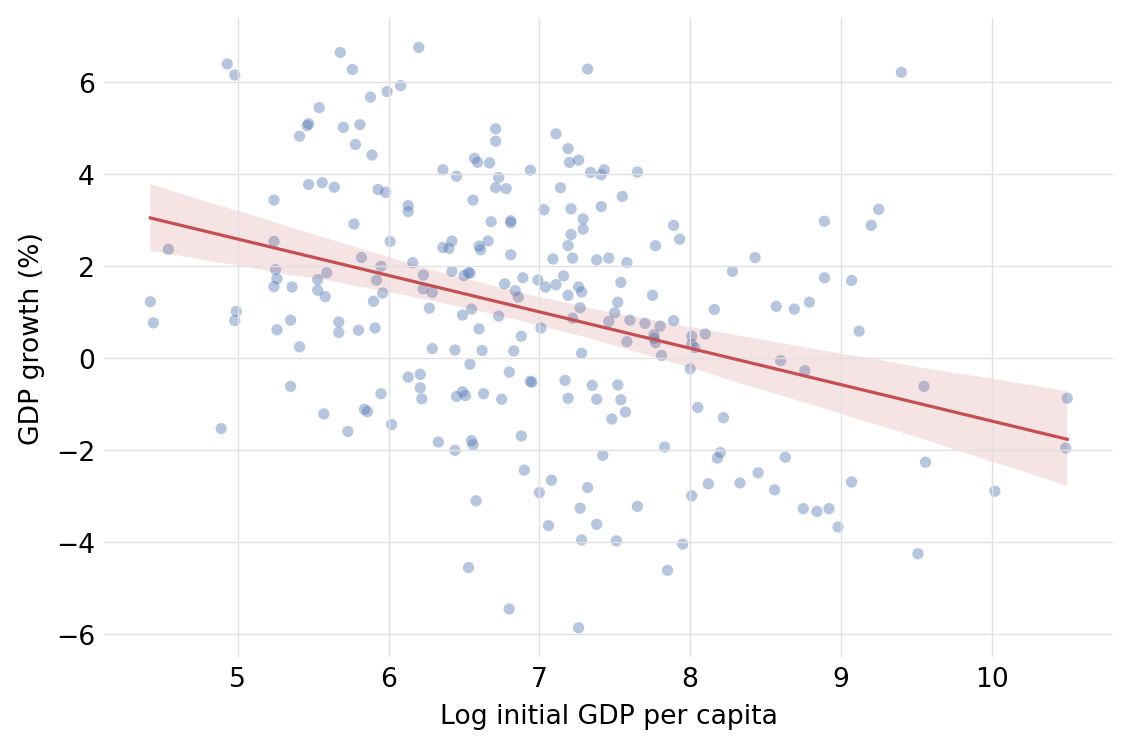
\includegraphics[keepaspectratio]{index_files/figure-latex/notebooks-notebook-01-fig-convergence-output-1.png}}

}

\caption{\label{fig-convergence}Conditional convergence: GDP growth
vs.~initial income level.}

\end{figure}%

The correlation structure of the panel variables is summarized below,
showing the pairwise relationships that motivate our regression
specification.

\begin{figure}[H]

\centering{

\pandocbounded{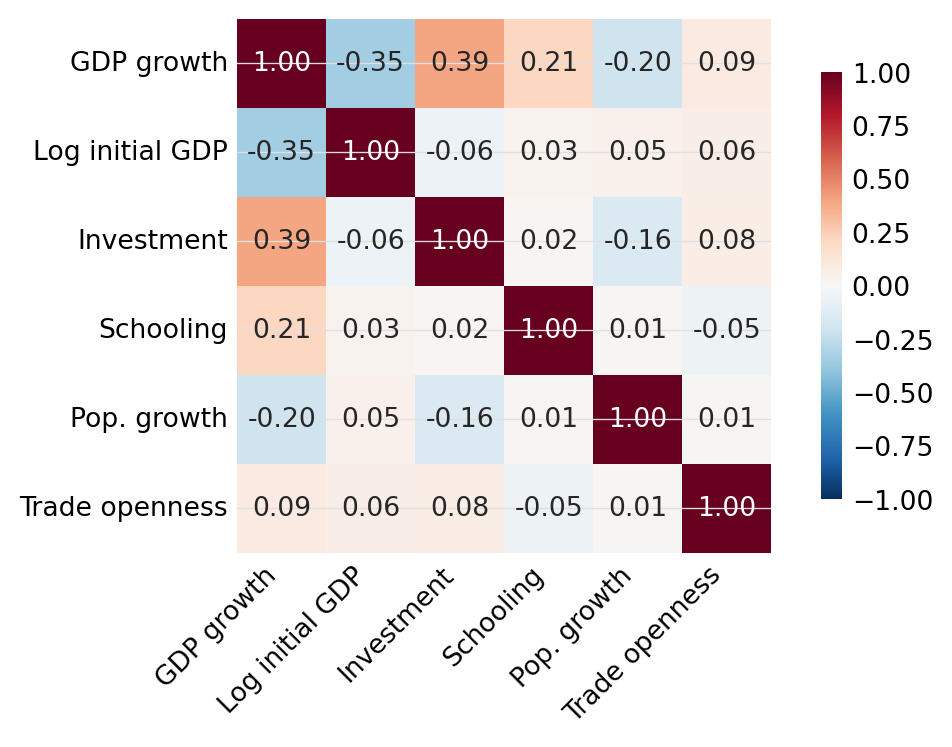
\includegraphics[keepaspectratio]{index_files/figure-latex/notebooks-notebook-01-fig-correlation-output-1.png}}

}

\caption{\label{fig-correlation}Pairwise correlations between panel
variables.}

\end{figure}%

The following table reports descriptive statistics at the beginning and
end of the sample period, highlighting how the panel evolves over time.

\textbf{Table 1: Descriptive statistics --- initial and final period.}

\begin{longtable}[]{@{}
  >{\raggedright\arraybackslash}p{(\linewidth - 12\tabcolsep) * \real{0.3380}}
  >{\raggedleft\arraybackslash}p{(\linewidth - 12\tabcolsep) * \real{0.1127}}
  >{\raggedleft\arraybackslash}p{(\linewidth - 12\tabcolsep) * \real{0.1408}}
  >{\raggedleft\arraybackslash}p{(\linewidth - 12\tabcolsep) * \real{0.0986}}
  >{\raggedleft\arraybackslash}p{(\linewidth - 12\tabcolsep) * \real{0.0986}}
  >{\raggedleft\arraybackslash}p{(\linewidth - 12\tabcolsep) * \real{0.0986}}
  >{\raggedleft\arraybackslash}p{(\linewidth - 12\tabcolsep) * \real{0.1127}}@{}}
\toprule\noalign{}
\begin{minipage}[b]{\linewidth}\raggedright
Variable
\end{minipage} & \begin{minipage}[b]{\linewidth}\raggedleft
Mean
\end{minipage} & \begin{minipage}[b]{\linewidth}\raggedleft
Median
\end{minipage} & \begin{minipage}[b]{\linewidth}\raggedleft
SD
\end{minipage} & \begin{minipage}[b]{\linewidth}\raggedleft
IQR
\end{minipage} & \begin{minipage}[b]{\linewidth}\raggedleft
Min
\end{minipage} & \begin{minipage}[b]{\linewidth}\raggedleft
Max
\end{minipage} \\
\midrule\noalign{}
\endhead
\bottomrule\noalign{}
\endlastfoot
GDP growth (1990) & -0.06 & 0.8 & 2.64 & 4.31 & -4.61 & 4.09 \\
GDP growth (2015) & 1.06 & 1.28 & 2.72 & 3.17 & -5.45 & 6.29 \\
Log initial GDP (1990) & 7.08 & 7 & 1.24 & 1.45 & 4.44 & 10.02 \\
Log initial GDP (2015) & 6.97 & 6.86 & 1.06 & 1.48 & 5.24 & 9.51 \\
Investment (1990) & 14.11 & 14.53 & 4.28 & 4.49 & 3.54 & 22.36 \\
Investment (2015) & 15.58 & 15.32 & 5.13 & 5.65 & 3.33 & 26.64 \\
Schooling (1990) & 5.91 & 5.5 & 3.36 & 4.93 & -1.23 & 13.15 \\
Schooling (2015) & 5.99 & 6.5 & 3.17 & 3.81 & -1.69 & 12.15 \\
Pop. growth (1990) & 1.55 & 1.54 & 0.57 & 0.54 & -0.01 & 2.97 \\
Pop. growth (2015) & 1.57 & 1.52 & 0.81 & 1.21 & 0.07 & 3.29 \\
Trade openness (1990) & 49.74 & 48.56 & 17.75 & 21.82 & 7.84 & 85.43 \\
Trade openness (2015) & 54.82 & 51.48 & 19.7 & 25.61 & 22.44 & 106.18 \\
\end{longtable}

\emph{Note:} Summary statistics for 40 countries at two points in time
(1990 and 2015). GDP growth in percentage points. Investment and trade
openness as shares of GDP. IQR = interquartile range.

\subsection{Methods}\label{methods}

We estimate the following growth equation using panel data fixed
effects:

\[
\text{Growth}_{it} = \beta_1 \ln \text{GDP}_{it} + \beta_2 \text{Investment}_{it} + \beta_3 \text{Schooling}_{it} + \beta_4 \text{PopGrowth}_{it} + \beta_5 \text{Trade}_{it} + \alpha_i + \gamma_t + \varepsilon_{it}
\]

where \(\alpha_i\) captures country fixed effects and \(\gamma_t\)
captures time fixed effects. We report four specifications: pooled OLS,
country FE, time FE, and two-way FE. Standard errors are clustered by
country in all models.

\section{Results and discussion}\label{sec-results}

The following table presents the main regression results estimated using
Python (\texttt{pyfixest}). We progressively add fixed effects to
control for unobserved heterogeneity.

\textbf{Table 2: Determinants of economic growth --- panel fixed effects
estimates (Python).}

\begin{longtable}[]{@{}lcccc@{}}
\toprule\noalign{}
& (1) OLS & (2) Country FE & (3) Time FE & (4) Two-way FE \\
\midrule\noalign{}
\endhead
\bottomrule\noalign{}
\endlastfoot
Log initial GDP & -0.759*** & -0.901*** & -0.742*** & -0.878*** \\
& (0.117) & (0.108) & (0.109) & (0.103) \\
Investment & 0.172*** & 0.200*** & 0.164*** & 0.190*** \\
& (0.030) & (0.025) & (0.028) & (0.024) \\
Schooling & 0.187*** & 0.168*** & 0.202*** & 0.186*** \\
& (0.044) & (0.040) & (0.048) & (0.038) \\
Pop. growth & -0.442** & -0.405** & -0.454*** & -0.431*** \\
& (0.169) & (0.159) & (0.159) & (0.151) \\
Trade openness & 0.013 & 0.014** & 0.015* & 0.017*** \\
& (0.009) & (0.006) & (0.008) & (0.006) \\
& & & & \\
Country FE & No & Yes & No & Yes \\
Year FE & No & No & Yes & Yes \\
Observations & 240 & 240 & 240 & 240 \\
R-squared & 0.332 & 0.641 & 0.381 & 0.687 \\
\end{longtable}

\emph{Note:} Dependent variable: GDP per capita growth rate (\%). All
regressions include a constant (not reported). Standard errors clustered
by country in parentheses. Significance levels: * p\textless0.10, **
p\textless0.05, *** p\textless0.01.

The results are replicated in R (\href{notebooks/notebook-02.qmd}{N2})
and Stata (\href{notebooks/notebook-03.qmd}{N3}) to demonstrate
multi-language reproducibility.

\textbf{Table 3: Determinants of economic growth --- panel fixed effects
estimates (R).}

\begin{longtable}[]{@{}lcccc@{}}
\toprule\noalign{}
& (1) OLS & (2) Country FE & (3) Time FE & (4) Two-way FE \\
\midrule\noalign{}
\endhead
\bottomrule\noalign{}
\endlastfoot
Log initial GDP & -0.759*** & -0.901*** & -0.742*** & -0.878*** \\
& (0.117) & (0.088) & (0.109) & (0.084) \\
Investment & 0.172*** & 0.200*** & 0.164*** & 0.190*** \\
& (0.030) & (0.027) & (0.028) & (0.024) \\
Schooling & 0.187*** & 0.168*** & 0.202*** & 0.186*** \\
& (0.044) & (0.037) & (0.048) & (0.036) \\
Pop. growth & -0.442** & -0.405** & -0.454*** & -0.431*** \\
& (0.169) & (0.168) & (0.159) & (0.152) \\
Trade openness & 0.013 & 0.014* & 0.015* & 0.017** \\
& (0.009) & (0.008) & (0.008) & (0.008) \\
& & & & \\
Country FE & No & Yes & No & Yes \\
Year FE & No & No & Yes & Yes \\
Observations & 240 & 240 & 240 & 240 \\
R-squared & 0.332 & 0.641 & 0.381 & 0.687 \\
\end{longtable}

\emph{Note:} Same specification as Table 2, estimated using R
\texttt{fixest}. All regressions include a constant (not reported).
Standard errors clustered by country.

\textbf{Table 4: Determinants of economic growth --- panel fixed effects
estimates (Stata).}

\begin{longtable}[]{@{}lcccc@{}}
\toprule\noalign{}
& (1) OLS & (2) Country FE & (3) Time FE & (4) Two-way FE \\
\midrule\noalign{}
\endhead
\bottomrule\noalign{}
\endlastfoot
Log initial GDP & -0.759*** & -0.901*** & -0.742*** & -0.878*** \\
& (0.117) & (0.088) & (0.109) & (0.084) \\
Investment & 0.172*** & 0.200*** & 0.164*** & 0.190*** \\
& (0.030) & (0.027) & (0.028) & (0.024) \\
Schooling & 0.187*** & 0.168*** & 0.202*** & 0.186*** \\
& (0.044) & (0.037) & (0.048) & (0.036) \\
Pop. growth & -0.442** & -0.405** & -0.454*** & -0.431*** \\
& (0.169) & (0.168) & (0.159) & (0.152) \\
Trade openness & 0.013 & 0.014* & 0.015* & 0.017** \\
& (0.009) & (0.008) & (0.008) & (0.008) \\
& & & & \\
Country FE & No & Yes & No & Yes \\
Year FE & No & No & Yes & Yes \\
Observations & 240 & 240 & 240 & 240 \\
Adj. R-squared & 0.318 & 0.560 & 0.354 & 0.607 \\
\end{longtable}

\emph{Note:} Same specification as Table 2, estimated using Stata
\texttt{reghdfe}. All regressions include a constant (not reported).
Standard errors clustered by country.

{[}FILL: Discuss implications and compare with existing literature.{]}

\section{Concluding remarks}\label{sec-conclusion}

{[}FILL: Summarize the main findings and their implications.{]}

{[}FILL: Discuss limitations and directions for future research.{]}

\section{Acknowledgments}\label{acknowledgments}

{[}FILL: Acknowledge funding sources, collaborators, and data
providers.{]}

\section{Data and code availability}\label{data-and-code-availability}

The data and code used in this study are available at {[}FILL:
repository URL{]}.

\section*{References}\label{references}
\addcontentsline{toc}{section}{References}

\phantomsection\label{refs}
\begin{CSLReferences}{1}{0}
\bibitem[\citeproctext]{ref-keola2015monitoring}
Keola, Souknilanh, Magnus Andersson, and Ola Hall. 2015. {``Monitoring
Economic Development from Space: Using Nighttime Light and Land Cover
Data to Measure Economic Growth.''} \emph{World Development} 66:
322--34.

\end{CSLReferences}




\end{document}
